\chapter{Introduction and Motivation}

Autonomous sensing systems increasingly need to make spatial decisions on small, power-limited platforms. A robot, drone, wearable device, or embedded sensor may need to estimate where an object is without relying on continuous cloud computation. In acoustic, sonar, or radar-like systems, this localisation problem means estimating range, horizontal angle (azimuth), and vertical angle (elevation) from reflected waves. The engineering challenge is therefore not only accuracy, but also how to structure the computation so that it is interpretable, robust, and potentially suitable for low-power hardware.

Spiking neural networks (SNNs) and neuromorphic hardware are promising in this context because they use event-like spikes and sparse communication rather than dense continuous activation at every timestep. Low-power operation is not directly measured in this project, so it is not claimed as a result. Instead, it provides the design motivation: if future sensing systems are to use neuromorphic hardware effectively, they need models whose computations are naturally event-driven and whose internal representations are meaningful enough to debug, test, and improve.

This project investigates whether biological structure is a useful way to design such an SNN-based sensing system. Rather than treating three-dimensional localisation as an end-to-end black-box regression task, the model is built from simplified functional analogues of the bat auditory system. Echolocating bats solve a closely related active-sensing problem: they emit short acoustic calls, receive returning echoes, and infer the three-dimensional structure of their environment in real time. The aim is not to reproduce a bat brain in biophysical detail, but to extract computational principles that can be implemented and tested in an engineering model.

The resulting system is a neuromorphic, bat-inspired model for active acoustic localisation. It emits a frequency-modulated call, simulates a returning binaural echo, converts the waveform into cochlear spike trains, processes distance, azimuth, and elevation through separate pathway models, and combines the resulting population codes using fixed readouts and a small trainable SNN. The central question is whether this bottom-up, interpretable, pathway-based architecture provides useful intermediate representations compared with less structured SNN baselines.

\section{Problem Specification}

The localisation task considered in this report is to estimate the spherical coordinate vector
\begin{equation}
    \mathbf{x} = (r, \theta, \psi),
\end{equation}
where $r$ is target distance, $\theta$ is azimuth, and $\psi$ is elevation. Figure~\ref{fig:intro_spherical_coordinates_redraft} shows this coordinate convention. The model observes the echo produced when an emitted acoustic signal reflects from a target. This can be viewed as a state-estimation problem: the hidden state is the target location, and the observation is a time-varying binaural waveform.

\begin{figure}[H]
    \centering
    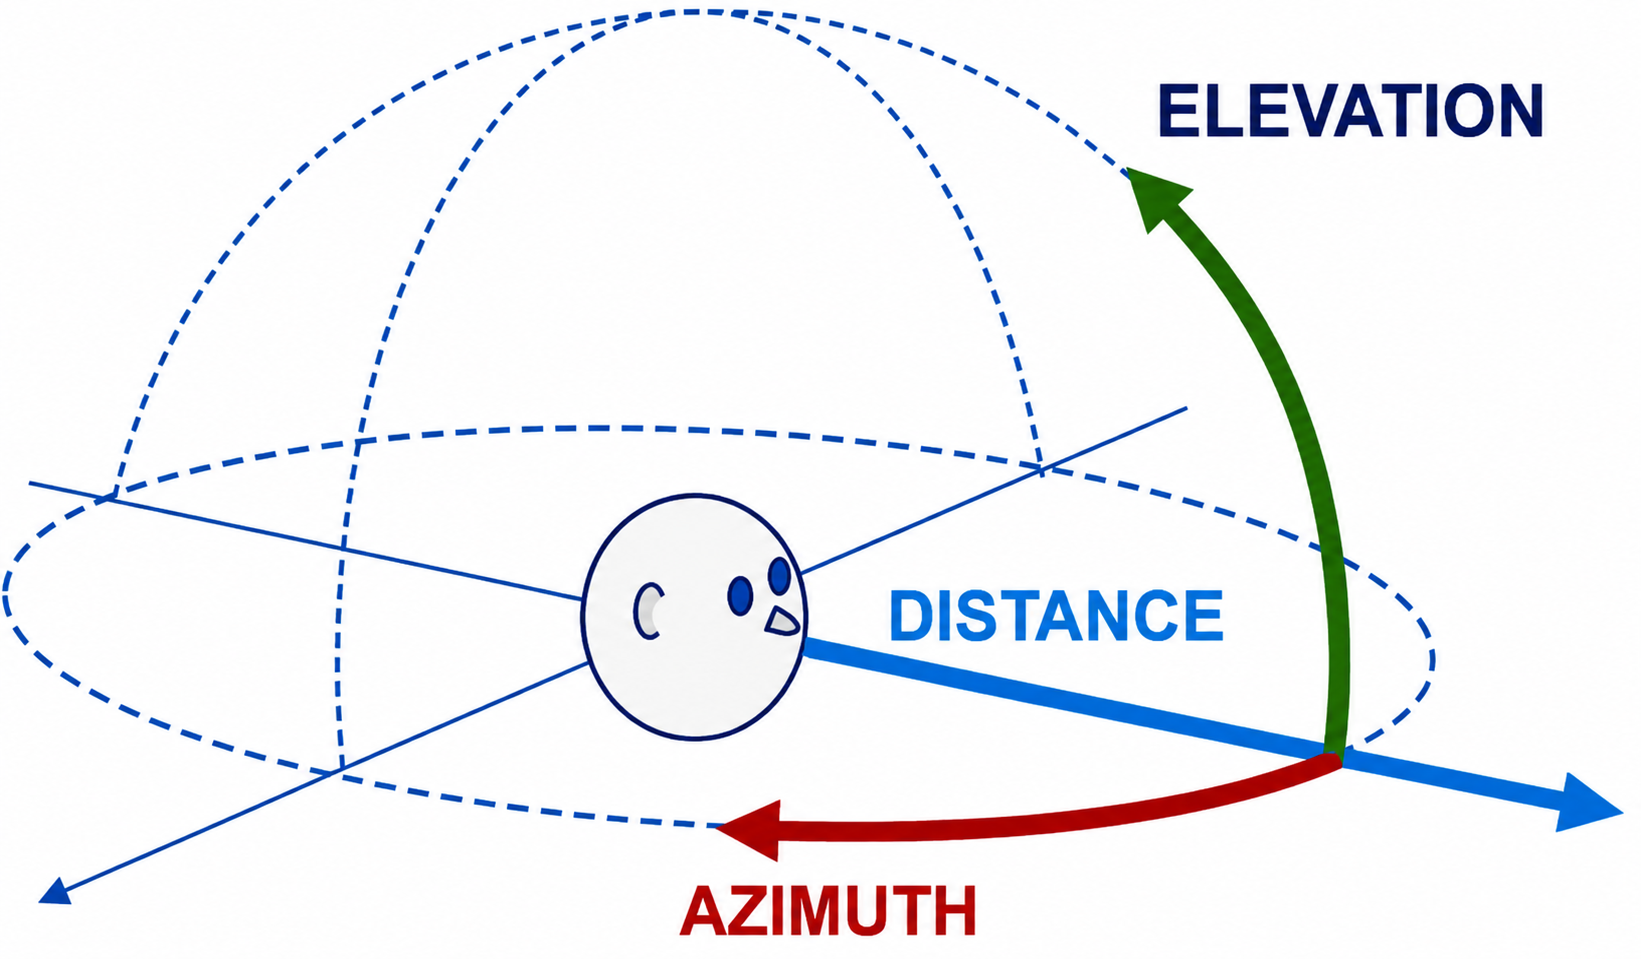
\includegraphics[width=0.70\linewidth]{1_Intro/intro_figures/polar_coords.png}
    \caption{Spherical coordinate representation of the localisation problem. The model estimates distance, azimuth, and elevation from the returning acoustic echo \cite{Carlini2024AuditoryReview}.}
    \label{fig:intro_spherical_coordinates_redraft}
\end{figure}

Conventional radar and sonar systems usually solve related localisation problems through explicit signal-processing pipelines, as illustrated in Figure~\ref{fig:intro_radar_redraft}. A radar system may perform range processing, Doppler processing, thresholding such as constant false alarm rate (CFAR) detection, and angle estimation, producing representations such as range-Doppler maps. These approaches are powerful and mathematically well understood, but they often rely on dense numerical operations over sampled signals. For high-performance radar or cloud-connected systems this cost may be acceptable. For small edge systems, it motivates asking whether a more event-driven and task-structured representation can reduce unnecessary computation.

\begin{figure}[H]
    \centering
    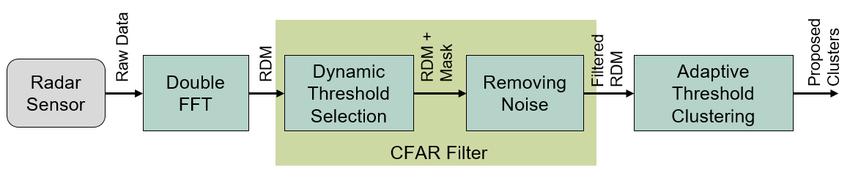
\includegraphics[width=0.70\linewidth]{1_Intro/intro_figures/radar_pipeline.png}
    \caption{Example radar processing pipeline. Conventional systems often use dense signal-processing stages before detection and object-level interpretation.}
    \label{fig:intro_radar_redraft}
\end{figure}

This report does not attempt to replace a full radar stack, nor does it compare against production radar algorithms. The radar analogy is used to clarify the type of problem being addressed: inferring object position from reflected waves. The implementation uses acoustic echoes because they are easier to simulate at biologically relevant timescales and because bat echolocation provides a strong biological model for active localisation.

\section{Why Use Biological Structure?}

Many SNN approaches are derived from conventional artificial neural networks: an ANN is trained and converted into an SNN, or a spiking architecture is trained directly using surrogate gradients. These methods can be effective, but they do not necessarily explain how to design the internal computation of a sensing system. A black-box SNN may use spikes, but it can still hide the physical structure of the task.

Biology suggests a different design route. The bat auditory system does not solve echolocation with one monolithic regression network. It decomposes the problem into specialised computations: cochlear frequency analysis, onset preservation, delay-sensitive coincidence detection, binaural comparison, spectral cue extraction, population coding, and spatial readout. These operations map naturally onto the physical cues in the echo. Distance is linked to pulse-echo delay, azimuth to differences between the ears, and elevation to direction-dependent spectral filtering by the outer ear.

This decomposition is attractive for two reasons. First, it produces interpretable intermediate representations: one can inspect the distance population, azimuth populations, elevation population, and readout estimates separately. Second, it provides a principled feature set for a final trainable SNN. Instead of asking a small network to discover all acoustic structure from raw waveforms, the model can provide biologically motivated pathway features and test whether those features improve the final readout.

Biology also provides an existence proof for efficient active sensing. Bats perform fast, closed-loop echolocation while flying and tracking prey, and the energy cost of echolocation has been measured to be low relative to the behavioural complexity of the task \cite{Speakman1989ThePipistrellus}. This does not prove that the software model developed here is low power. It does, however, motivate looking beyond generic neural networks toward event-driven, biologically structured computation.

\section{Aims and Objectives}

The overall aim of the project is to test whether a three-dimensional active-acoustic localisation problem can be solved using a structured neuromorphic model inspired by the bat auditory system. More specifically, the project asks whether biologically motivated pathways provide useful intermediate representations for distance, azimuth, and elevation, and whether those representations improve a small trainable SNN readout compared with less structured inputs.

The main objectives are:
\begin{itemize}
    \item to construct a simulated active-acoustic environment in which an emitted frequency-modulated call produces distance, azimuth, and elevation cues in the returning binaural echo;
    \item to develop a cochlear spike front end that converts the acoustic waveform into an event-based, frequency-organised representation;
    \item to build separate distance, azimuth, and elevation pathways using simplified biological computations, including delay coincidence, binaural comparison, and spectral-template matching;
    \item to compare direct centre-of-mass readouts, calibrated readouts, and SC-style continuous-attractor readouts for pathway population codes;
    \item to train SNN readouts on the pathway-derived feature set and compare them with SNN baselines trained from less structured inputs such as raw binaural waveforms or cochlear spike rasters;
    \item to evaluate the final model under noise-free, environmental-noise, and delayed-echo conditions, while identifying the limits of the constrained operating region.
\end{itemize}

The contribution is therefore a complete modelling pipeline rather than a single isolated algorithm. The work shows how an active sensing task can be decomposed into interpretable neuromorphic components, how those components can be tested individually, and how a limited trainable readout can be added without discarding the biological structure. The final design principle is hybrid: fixed biomimetic pathways provide interpretable feature extraction, while a small trainable SNN performs contextual integration and residual correction.

\section{Report Structure}

Chapter 2 provides the biological and neuromorphic background needed to understand the model. It introduces auditory localisation cues, echolocation, spiking computation, coincidence detection, population codes, and the auditory pathways used as inspiration.

Chapter 3 describes the modelling and implementation. It explains the acoustic simulation, cochlear front end, distance pathway, azimuth pathway, elevation pathway, SC-style readouts, and trainable fusion network.

Chapter 4 presents the results. It evaluates the fixed pathway readouts, trainable SNN readouts, input baselines, robustness to noise and delayed echo components, and the main error structure of the final model.

Chapter 5 concludes the report by summarising the main findings, discussing limitations, and identifying future work needed to move from this prototype toward a more complete neuromorphic echolocation system.
